\section{Theoretische Grundlagen}

%Zerfallskaskaden
%Wirkungsweise von Szintillationszählern und Photomultipliern
%Zufällige Koinzidenzen

\subsection{$\alpha$-Zerfall}

Zerfällt ein sogenannter Mutterkern $_Z^AX$ in einen Tochterkern $_{Z-2}^{A-4}Y$ und ein $He^{2+}$-Ion so spricht man von $\alpha$-Zerfall. Das $He^{2+}$-Teilchen wird $\alpha$-Teilchen genannt. Die Emission von $\alpha$-Teilchen ist ein quantenmechanischer Prozess, der durch das Tunneln des $\alpha$-Teilchens durch die Potentialbarriere des Coulombpotentials des Kerns ermöglicht wird. $\alpha$-Teilchen zeigen ein diskretes Spektrum und sind monochromatisch.

\subsection{$\beta$-Zerfall}

Man unterscheidet beim $\beta$-Zerfall zwischen $\beta^+$- und $\beta^-$-Zerfall. Der $\beta^+$-Zerfall ist die Umwandlung eines Protons in ein Neutron mit Emission eines Positrons und eines Elektronenneutrinos:

$$ \beta^+: p^+ \rightarrow n^0 + e^+ + \nu_e $$

Der $\beta^-$-Zerfall hingegen, ist die Umwandlung eines Neutrons in ein Proton, unter Emission eines Elektrons und eines Elektron-Antineutrinos:

$$ \beta^-: n^0 \rightarrow p^+ + e^- + \bar \nu_e $$

Der $\beta^+$-Zerfall ist nur möglich für Protonen in einem Kern, da durch die Bindungsenergie die für den Prozess nötige Energie aufgebracht werden kann.

Als weitere Art des $\beta$-Zerfall zählt man noch den Elektroneneinfang (EC, \emph{electron capture)}. Dieser kann stattfinden, wenn ein Elektron der untersten Schale (K-Schale), wegen dessen Aufenthaltswahrscheinlichkeit im Kern, vom Kern eingefangen wird und mit einem Proton zu einem Neutron wird unter Emission eines Elektronenneutrinos:

$$ EC: p^+ + e^- \rightarrow n^0 + \nu_e $$

Der Elektroneneinfang gewinnt mit größeren Kernzahlen an Bedeutung, da dann die Aufenthaltswahrscheinlichkeit im Kern immer größer wird.

\subsection{$\gamma$-Strahlung}

Beim $\alpha$- und $\beta$-Zerfall gehen die Mutterkerne immer mit bestimmten Wahrscheinlichkeiten in verschiedene Zustände der Tochterkerne über. Letztere zerfallen innerhalb einer sehr kurzen Zeit ($\sim 10^-9 bis 10^-12 s$) in den Grundzustand und emittieren dabei ein Photon, genannt $\gamma$-Quant. Dieses $\gamma$-Quant wird entweder direkt vom Kern emittiert oder kann durch folgende Prozesse induzieren:

\subsubsection{Innere Konversion}

Die Energie des Kerns geht an ein Hüllenelektron, welches dadurch das Atom mit der verbleibenden Energie als kinetische Energie verlässt. Diese Elektronenlücke wird durch ein Elektron aus einer höheren Schale ersetzt, welches diesen Energieverlust durch ein Photon (bei schweren Elementen) oder den Auger-Effekt (bei leichten Elementen) kompensiert.

\subsubsection{Der Auger-Effekt}

Falls dieses oben erklärte Elektron dieses Loch füllt, kann es sein, dass die überschüssige Energie wiederum an ein Elektron abgegeben wird, welches dadurch das Atom verlässt und damit ein zweites Loch im Atom hinterlässt.


\subsection{Wechselwirkung von Photonen mit Materie}

\subsubsection{Das Absorptionsgesetz}

Ein Photonenstrahl der einfallenden Intensität $I_0$ nimmt exponentiell mit der Dicke x einer durchquerten Materieschicht an Intensität ab. Es gilt also:

$$ I = I_0\cdot e^{-\mu x} $$

wobei $\mu$ der mediumabhängige (und photonenenergieabhängige) Absorptionkoeffizient ist. $\mu$ lässt sich als Summe der Absorptionskoeffizienten aller möglichen Wechselwirkungen von Photonen mit Materie schreiben, nämlich des Photoeffekts, des Compton-Effekts und der Paarbildung.

$$\mu = \mu_{Ph.} + \mu_{C} + \mu_{PB} $$

\subsubsection{Der Photoeffekt}

\begin{figure}[H]
	\begin{minipage}{0.6\textwidth}
	\centering 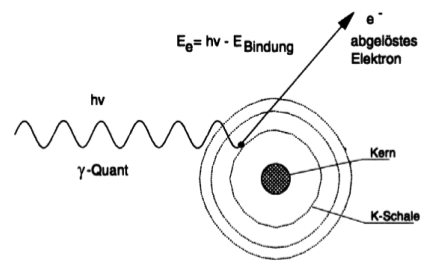
\includegraphics[width=\textwidth]{Bilder/Photoeffekt.png}
	\caption{Photoeffekt}
	\end{minipage}
	\begin{minipage}{0.4\textwidth}
	Wenn ein $\gamma$-Quant ein Elektron aus der Atomhülle herausschlägt, spricht man vom Photoeffekt. 	Dieser Effekt tritt also nur an gebundenen Elek\-tro\-nen auf. Die Energie des Photons geht zum größten Teil 	auf das Elektron, ein Teil wird jedoch als Rückstoßenergie vom Atom aufgenommen. Die 				Ab\-sorp\-tions\-wahrscheinlichkeit ist am größten in der K-Schale, also näher beim Kern. Der Photoeffekt 	dominiert gegenüber den anderen Effekten vor allem bei großen Atomen und Energien unter 100keV des	Photons. Nach dem Ablösen des Elektrons strahlt das ionisierte Atom die Bindungsenergie wieder ab.
	\end{minipage}
\end{figure}

\subsubsection{Der Compton-Effekt}

\begin{figure}[H]
	\begin{minipage}{0.4\textwidth}
	Trifft ein Photon auf ein leicht gebundenes oder freies Elektron, so wird das Photon nicht ganz absorbiert, sondern gibt einen Teil seiner Energie an das Elektron ab und wird selbst gestreut. Durch die Streuung verliert das Photon somit an Energie, d.h. die Frequenz des gestreuten Quants ist kleiner. Der Compton-Effekt dominiert bei Energien zwischen 100 keV und einigen MeV.
	\end{minipage}
	\begin{minipage}{0.6\textwidth}
	\centering 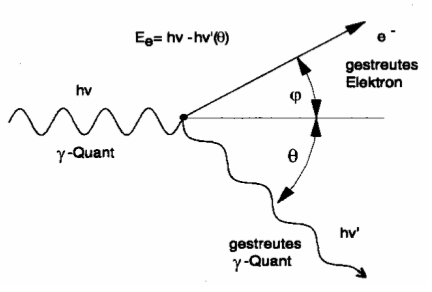
\includegraphics[width=\textwidth]{Bilder/Comptoneffekt.png}
	\caption{Comptoneffekt}
	\end{minipage}

\end{figure}

\subsubsection{Die Paarbildung}

\begin{figure}[H]
	\begin{minipage}{0.5\textwidth}
	\centering 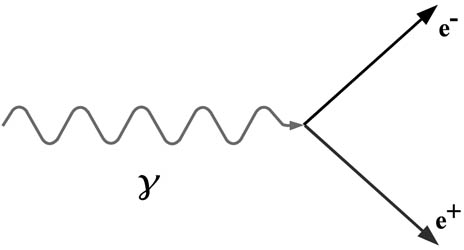
\includegraphics[width=\textwidth]{Bilder/Paarbildung.jpg}
	\caption{Paarbildung}
	\end{minipage}
	\begin{minipage}{0.5\textwidth}
	Hat der $\gamma$-Quant mindestens die doppelte Ruheenergie eines Elektrons, also 1.022 MeV, so kann dieses im Feld eines Atomkerns (Stoßpartner für die Energie-Impuls-Erhaltung) ein Elektron-Positron-Paar erzeugen. Das Positron kann in Anwesenhait von Materie nicht frei existieren und wird abgebremst und annihiliert mit einem Elektron zu 2 bis 3 $\gamma$-Quanten. Im wahrscheinlicheren Fall zweier Quanten, erhalten diese jeweils eine Energie von 511 keV und bewegen sich in einem Winkel von 180° relativ zueinander (Impulserhaltung).
	\end{minipage}
\end{figure}






























